\documentclass[border=10pt]{standalone}

\usepackage{tikz}
\usepackage{tikzsymbols}
\usetikzlibrary{calc,patterns,shapes.geometric}

\def\centerarc[#1](#2)(#3:#4:#5){\draw[#1] ($(#2)+({#5*cos(#3)},{#5*sin(#3)})$) arc (#3:#4:#5);}

\begin{document}
	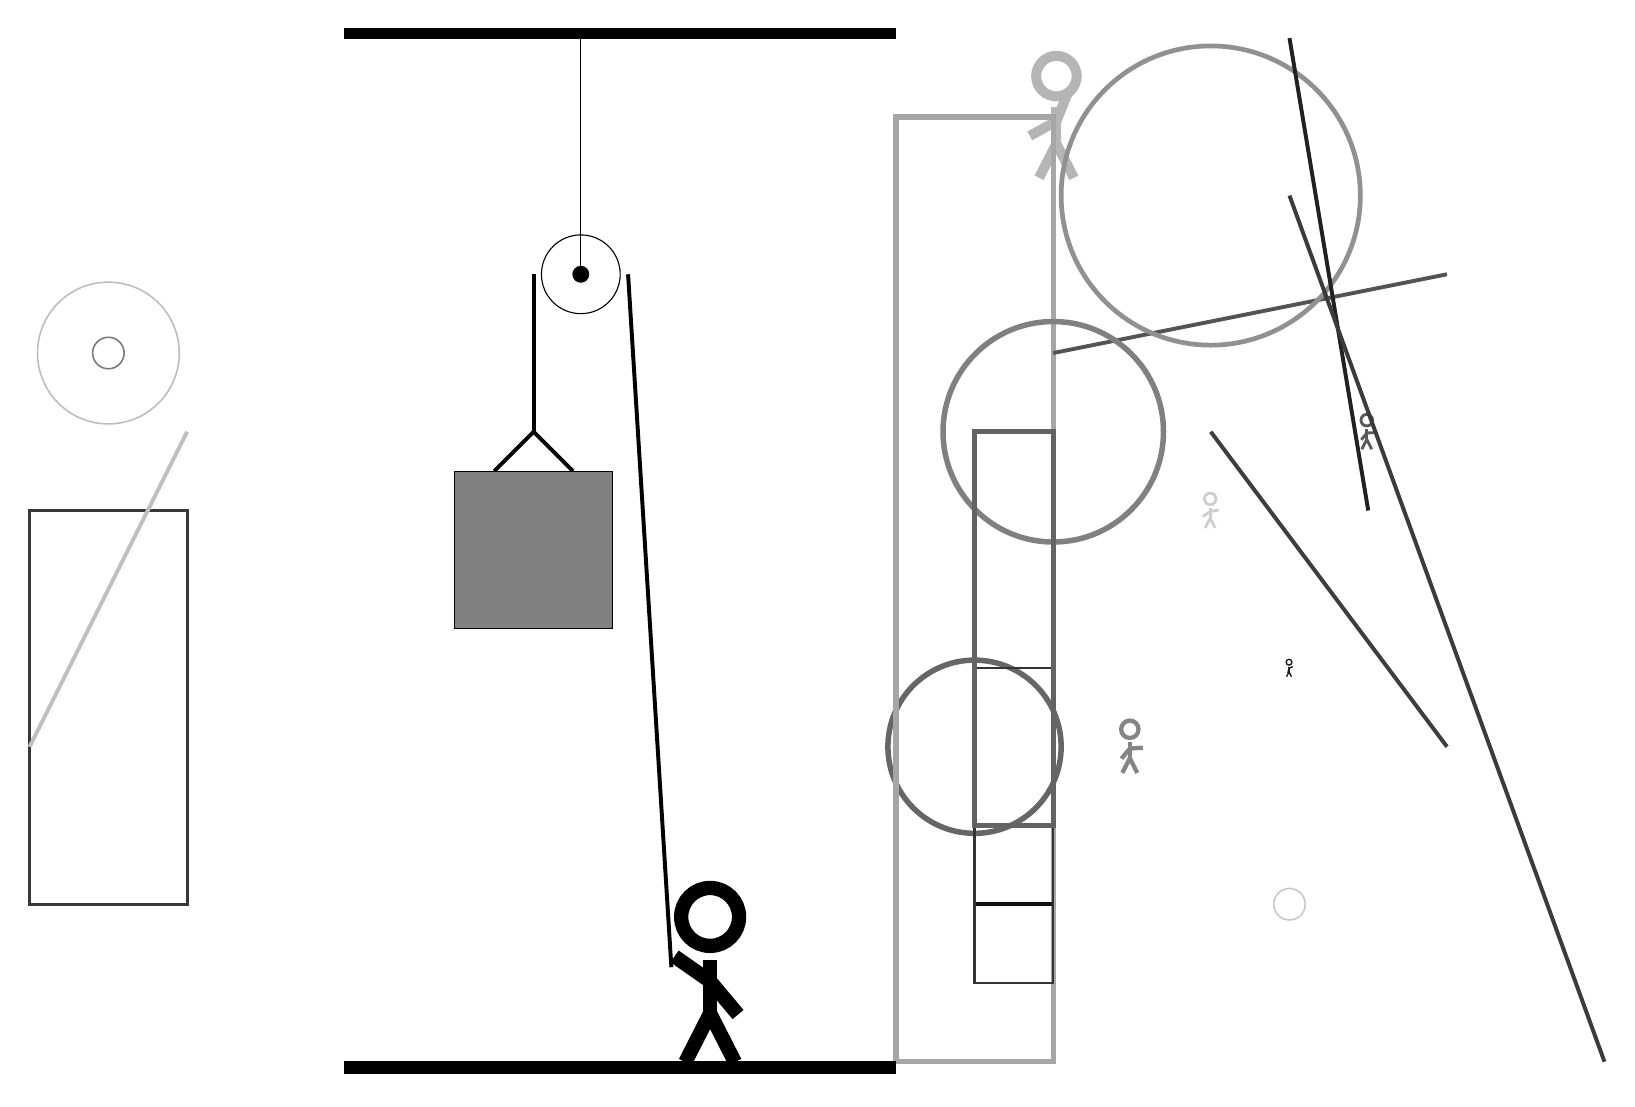
\begin{tikzpicture}
		%%%%% START %%%%%
		
		\draw[fill=black] (-2, 10) rectangle (5, 10.125);
		
		\draw[line width=0.5mm, color=black!76](9, 5) -- (12, 1);
		
		\draw[line width=0.4mm, color=black!78] (-4, -1) rectangle (-6, 4);
		\node[line width=0.2mm, color=black!29] at (7, 9) {\Strichmaxerl[7][29][68]};
		\draw [line width=0.7mm, color=black!60](6, 1) circle (1.1);
		\draw[line width=0.7mm, color=black!35] (5, 9) rectangle (7, -3);
		\draw[line width=0.5mm, color=black!25](-4, 5) -- (-6, 1);
		\node[line width=0.2mm, color=black!88] at (10, 2) {\Strichmaxerl[1][74][30]};
		
		\node[line width=0.4mm, color=black!19] at (9, 4) {\Strichmaxerl[2][33][13]};
		\draw[line width=0.5mm, color=black!67](7, 6) -- (12, 7);
		
		\draw[line width=0.5mm, color=black!94] (6, -1) rectangle (7, -1);
		
		\draw [line width=0.2mm, color=black!22](10, -1) circle (0.2);
		\draw [line width=0.2mm, color=black!53](-5, 6) circle (0.2);
		\node[line width=0.2mm, color=black!65] at (11, 5) {\Strichmaxerl[2][51][3]};
		
		\draw [line width=0.6mm, color=black!43](9, 8) circle (1.9);
		\node[line width=0.2mm, color=black!48] at (8, 1) {\Strichmaxerl[3][50][4]};
		\draw[line width=0.3mm, color=black!80] (7, -2) rectangle (6, 2);
		\draw [line width=0.7mm, color=black!50](7, 5) circle (1.4);
		
		\draw[line width=0.5mm, color=black!87](10, 10) -- (11, 4);
		\draw[line width=0.5mm, color=black!77](10, 8) -- (14, -3);
		\draw[line width=0.6mm, color=black!61] (6, 0) rectangle (7, 5);
		\draw [line width=0.2mm, color=black!26](-5, 6) circle (0.9);
		
		
		\draw (1, 7) circle (0.5);
		\draw[fill=black] (1, 7) circle (0.1);
		\draw (1, 10) -- (1, 7);
		
		\draw[line width=0.5mm] (-0.1, 4.5) -- (0.4, 5.0) -- (0.9, 4.5);
		\draw[fill=black!50] (-0.6, 4.5) rectangle (1.4, 2.5);
		
		\draw[line width=0.5mm] (0.4, 7) -- (0.4, 5.0);
		\centerarc[line width=0.5mm](1, 7)(0:180:0.6);
		\draw[line width=0.5mm](1.6, 7) -- (2.15, -1.8);
		
		\node at (2.6, -1.9) {\Strichmaxerl[10][-35][-50]};
		
		\draw[fill=black] (-2, -3) rectangle (5, -3.15);
		
		%%%%% END %%%%%
	\end{tikzpicture}
\end{document}